% \documentclass[10pt, draft]{beamer}
% \documentclass[10pt, handout]{beamer}
\documentclass[10pt]{beamer}
\usetheme[
	% sectionpage=progressbar,
	% subsectionpage=progressbar,
	progressbar=head]{metropolis}

\useoutertheme{infolines}
% \useinnertheme{rounded}
\usecolortheme{beaver}



\usepackage{longtable}
\usepackage{newtxtext,newtxmath}
\usepackage[backend=biber,style=gb7714-2015, gbnamefmt=lowercase, 
maxcitenames=2,
mincitenames=1, 
gbcitelocal=gb7714-2015,
gbpub=false,
doi=false,
isbn=false,
url=false,
eprint=false]{biblatex}
\addbibresource{yy.bib}
\hypersetup{pdfpagemode=FullScreen}
\usepackage{ctex}
\setmainfont{Times New Roman}
\setCJKmainfont[ItalicFont=华文楷体,BoldFont=华文细黑]{华文宋体}
\usepackage{graphicx}
\usepackage{amsmath}
\usepackage{amsfonts}
\usepackage{subfigure}
\usepackage{url}
\definecolor{awesome}{rgb}{1.0, 0.13, 0.32}
% \usepackage{mathptm}
\numberwithin{equation}{section}
\usefonttheme[onlymath]{serif}
% \setlength{\parskip}{1.2em}
\DeclareGraphicsExtensions{.eps,.ps,.jpg,.bmp,.png}

\author{统计71~~王泽昊}
\institute{指导教师: 张春霞}

\date{2021年4月21日}

\title{数学与统计学院~毕业设计}
\subtitle[本科毕业设计]{聚类算法在地震速度谱自动拾取中的应用研究}

\graphicspath{{images/}}


\begin{document}

{\usebackgroundtemplate{
\includegraphics[height=\paperheight,width=\paperwidth]{background.png}}
\maketitle

\begin{frame}
    \frametitle{目录}
    \bfseries
    \large
    \begin{itemize}
        \item 问题背景
        \vspace{5pt}\item 理论知识
        \begin{itemize}
            \vspace{5pt}\item K-means
            \item DBSCAN
            \item 基于EM算法的GMM
            \item 变分推断
            \item 基于Dirichlet过程的高斯混合模型
        \end{itemize}
        \vspace{5pt}\item 数值实验
        \begin{itemize}
            \vspace{5pt}\item 不同聚类算法结果对比
            \item 地震原始记录拉直
        \end{itemize}
        \vspace{5pt}\item 结论与展望
    \end{itemize}
\end{frame}

\section{问题背景}

% \begin{frame}[c]
%     \frametitle{背景知识学习}
%         \begin{figure}[h]
%             \centering
%             \includegraphics[width = .3\textwidth]{Book.jpg}
%         \end{figure}
%         由于地震勘探学背景知识的缺乏, 对此书籍\footfullcite{Zhou2014}的前四章进行了学习. 
% \end{frame}

\begin{frame}[c]
    \frametitle{CMP道集}
    \begin{minipage}{.55\paperwidth}
        \begin{figure}[h]
            \centering
            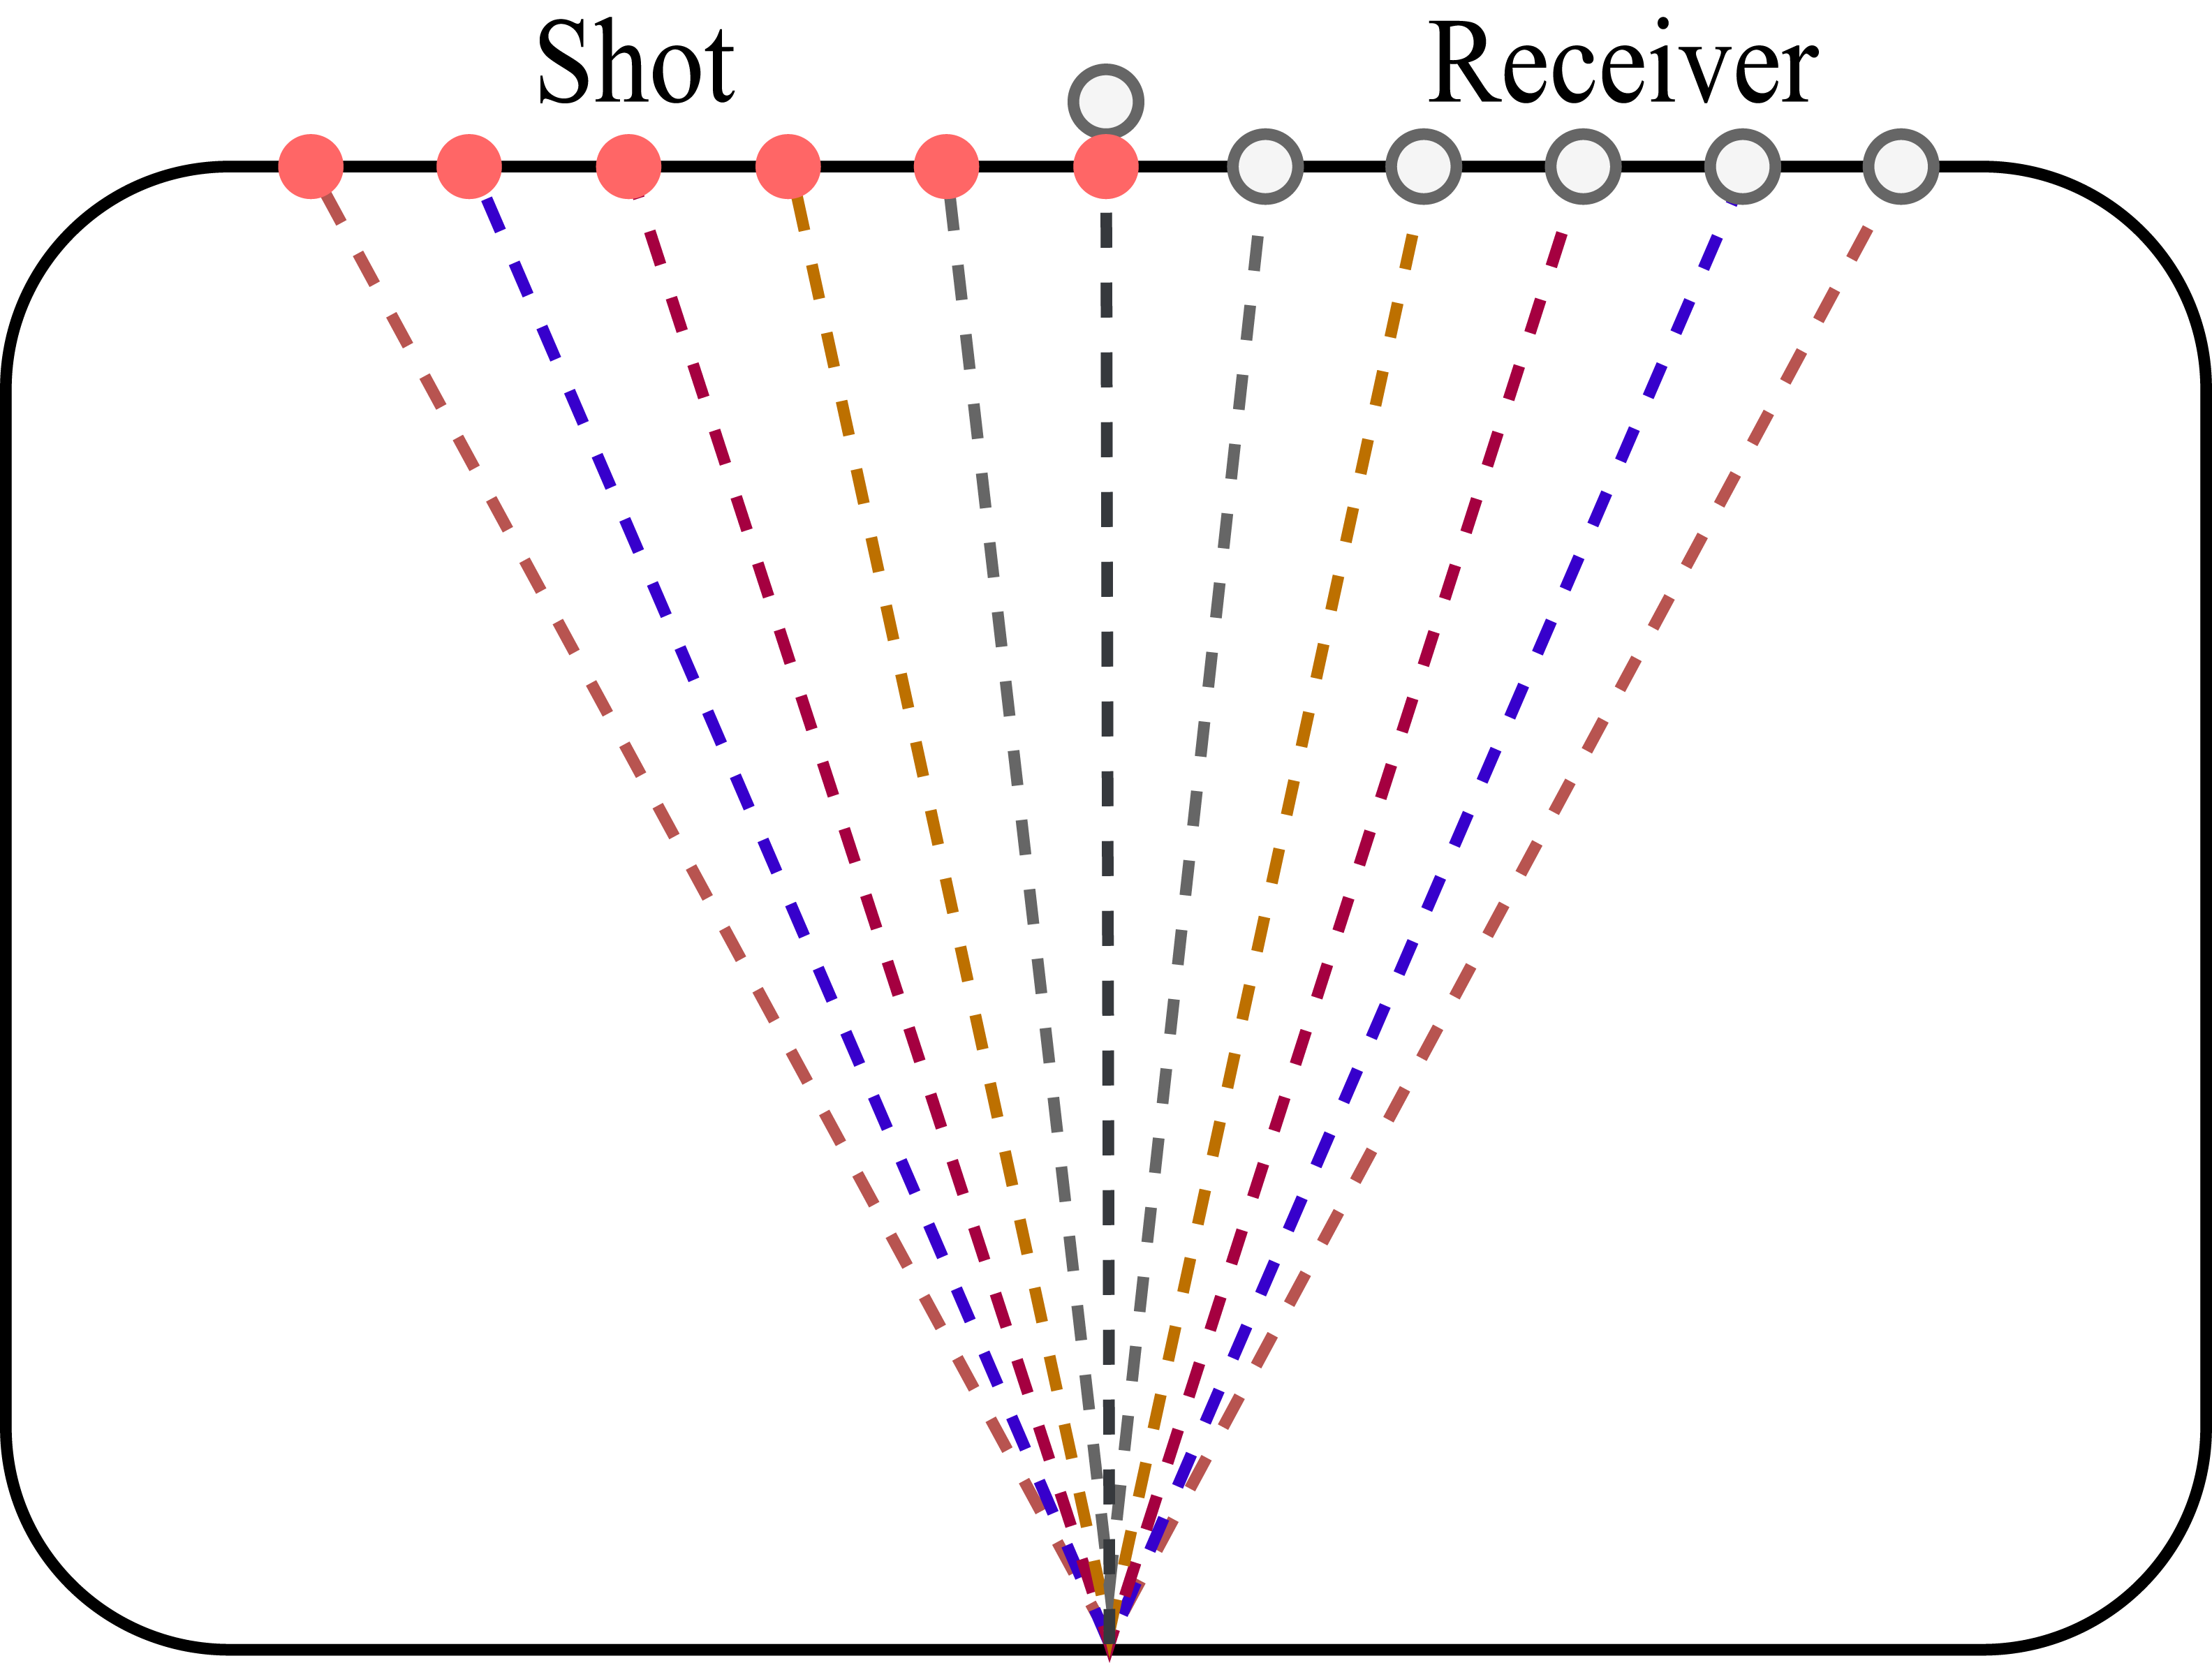
\includegraphics[width = .9\textwidth]{03_共中点道集.png}
            \caption{共中心点道集检波器布局}
        \end{figure}
    \end{minipage}
    \begin{minipage}{.35\paperwidth}
        Shot代表激发器, Receiver代表接收器, 每一对Shot-Receiver都呈对称分布. 
    \end{minipage}
\end{frame}

\begin{frame}[c]
    \frametitle{对应的速度谱}
    \begin{minipage}{.55\paperwidth}
        \begin{figure}[h]
            \centering
            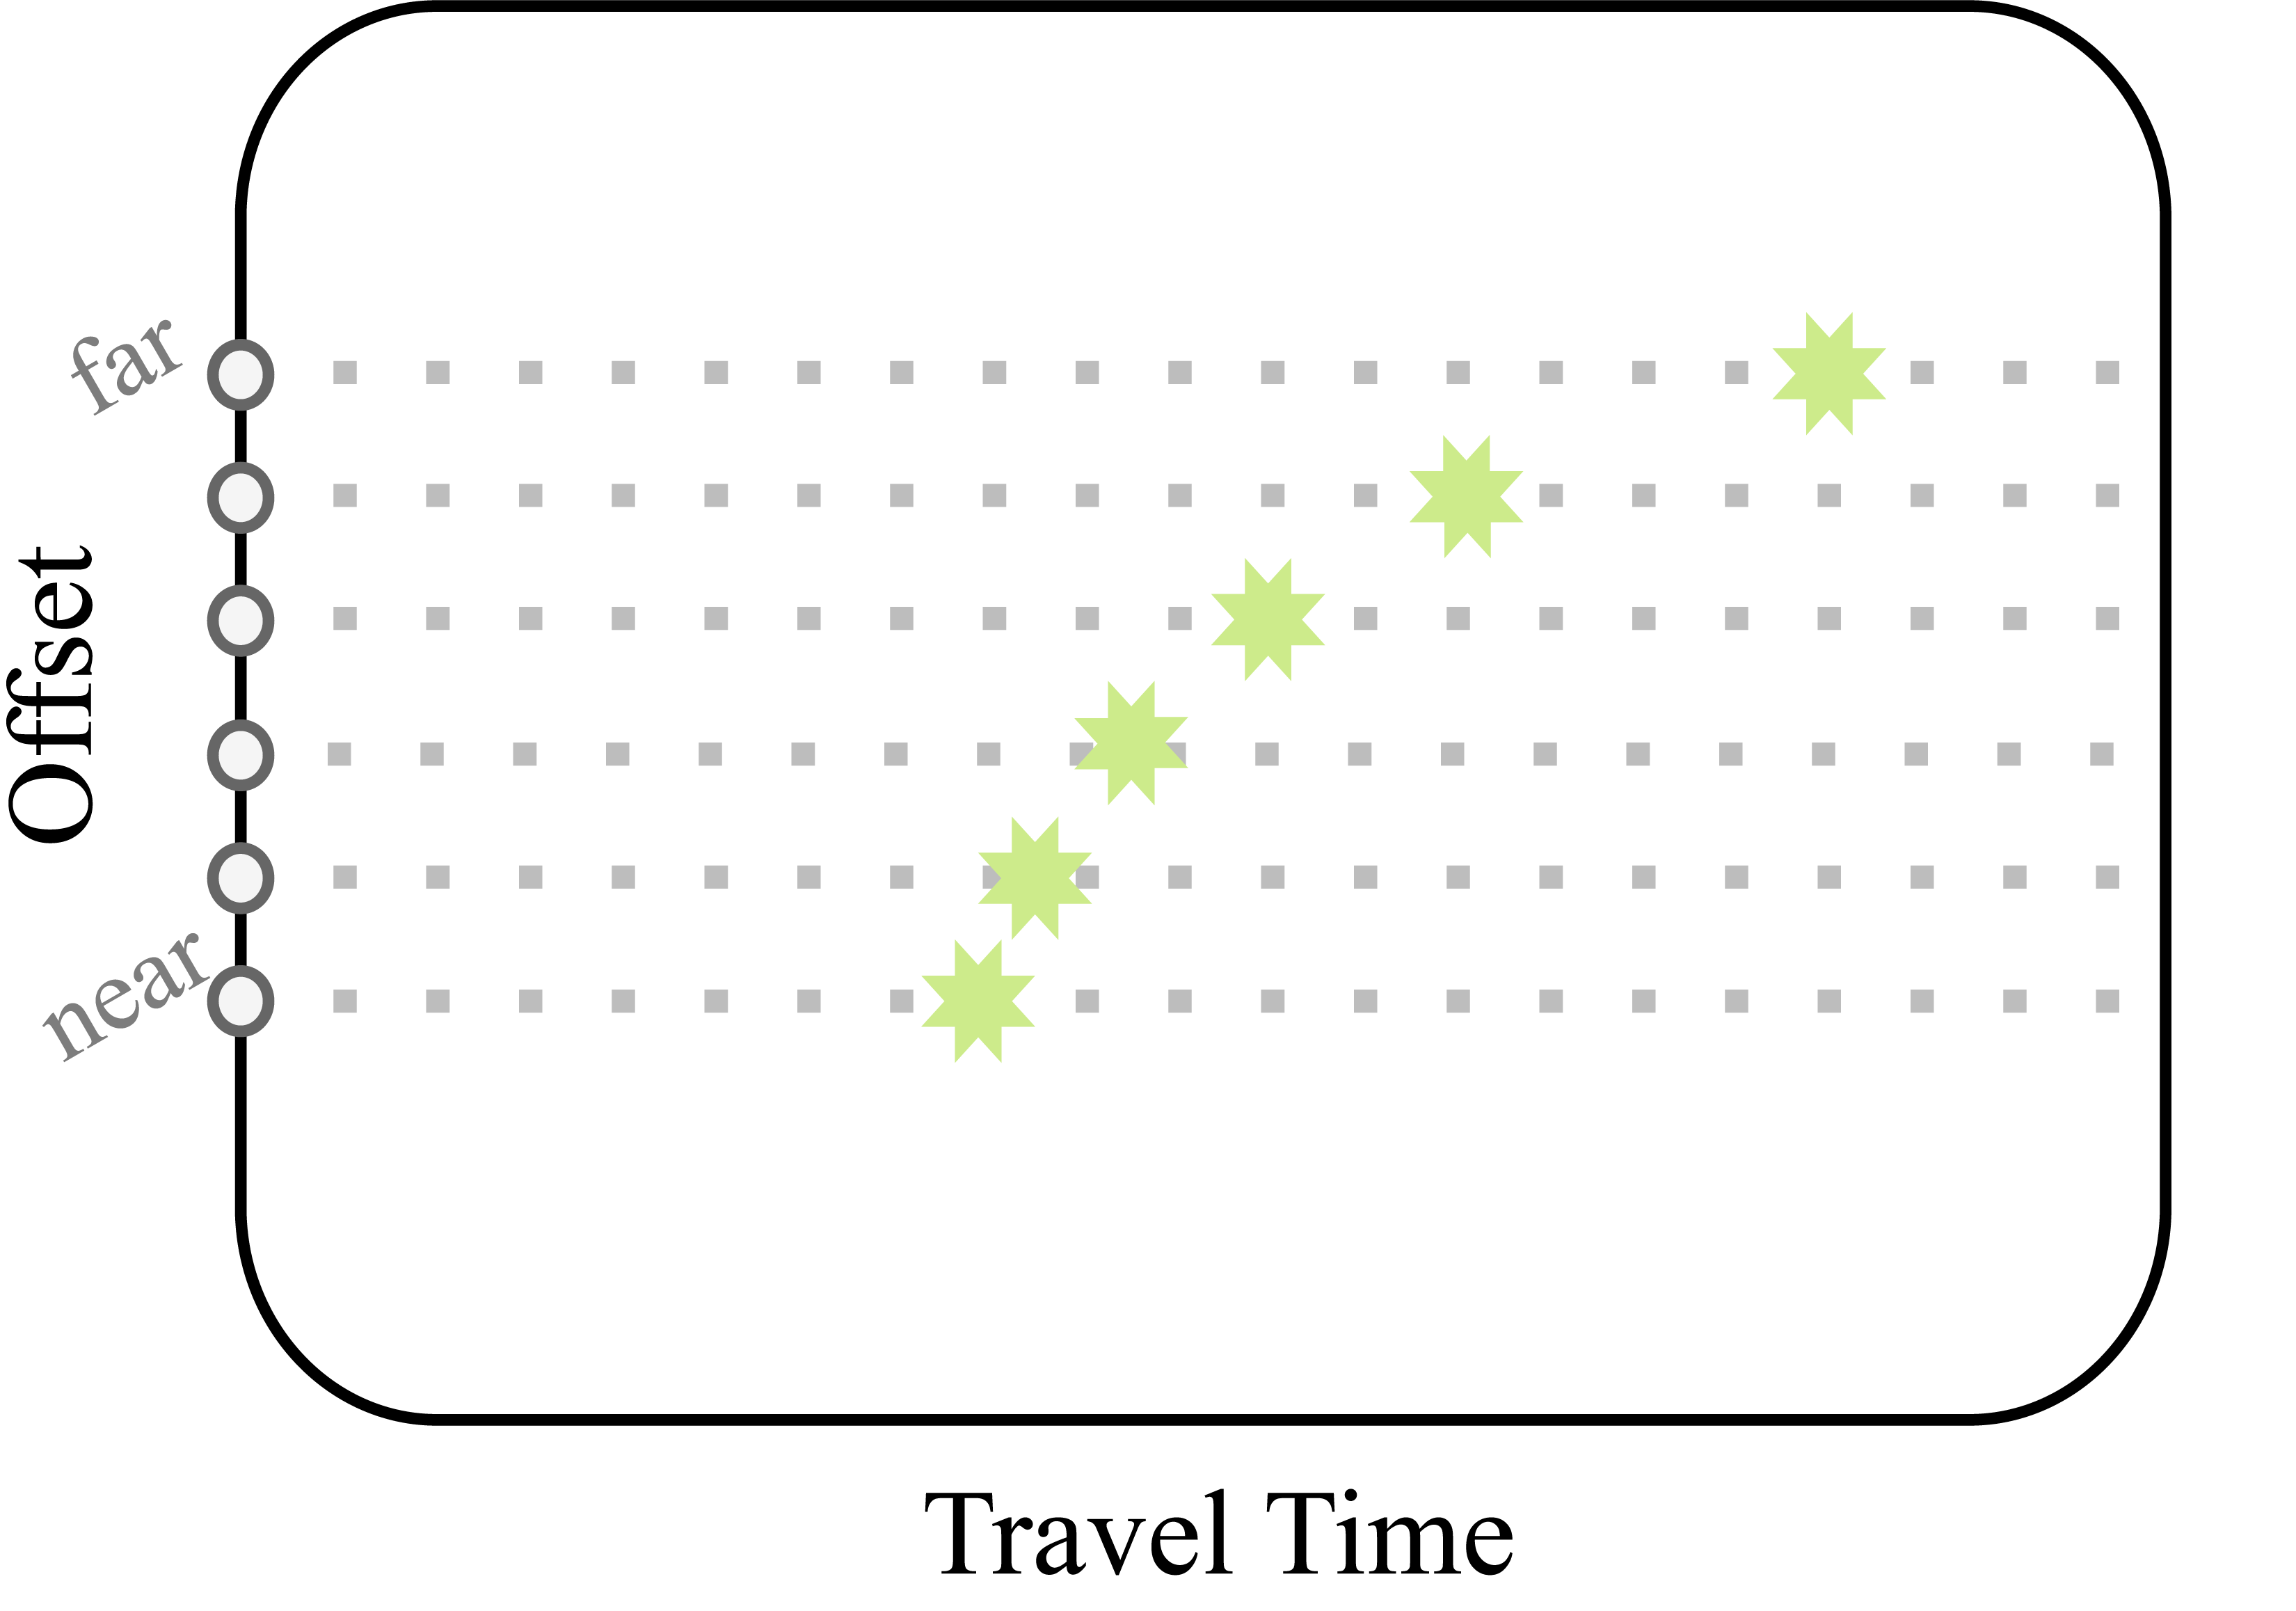
\includegraphics[width = .9\textwidth]{04_偏移距与旅行时图像_NMO前.png}
            \caption{地震信号传播的距离跟旅行时之间的关系}
        \end{figure}
    \end{minipage}
    \begin{minipage}{.35\paperwidth}
        Offset为偏移距, 即Shot-Receiver间的水平距离; Travel Time为旅行时, 即Shot发出的信号被Receiver接收到所需的时间. 
    \end{minipage}
\end{frame}

\begin{frame}[c]
    \frametitle{动校正介绍}
        \begin{figure}[h]
            \captionsetup{justification=centering}
            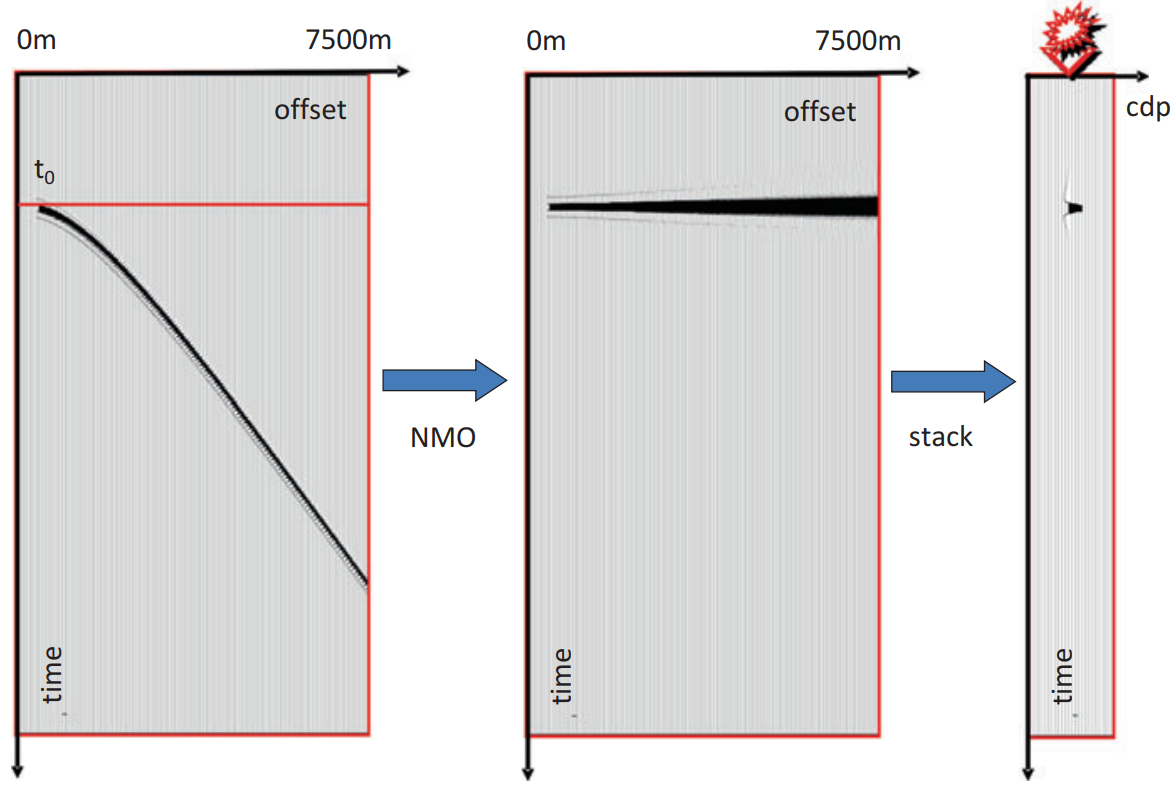
\includegraphics[width=.7\textwidth]{01_动校正过程.png}
            \caption{原始速度谱到动校正后的速度谱再到叠加后的速度谱, \\速度谱拾取是动校正中一个重要的环节}
        \end{figure}
\end{frame}

\begin{frame}[c]
    \frametitle{动校正}
    偏移距: $x$, 旅行时: $t$, 传播长度: $l$, 反射点深度: $h$, 零偏移距旅行时: $t_0$, 波速: $v$, 可以计算得到\footfullcite{Zhou2014}

    \vspace{10pt}
    \begin{minipage}{.55\paperwidth}
        \begin{figure}[h]
            \centering
            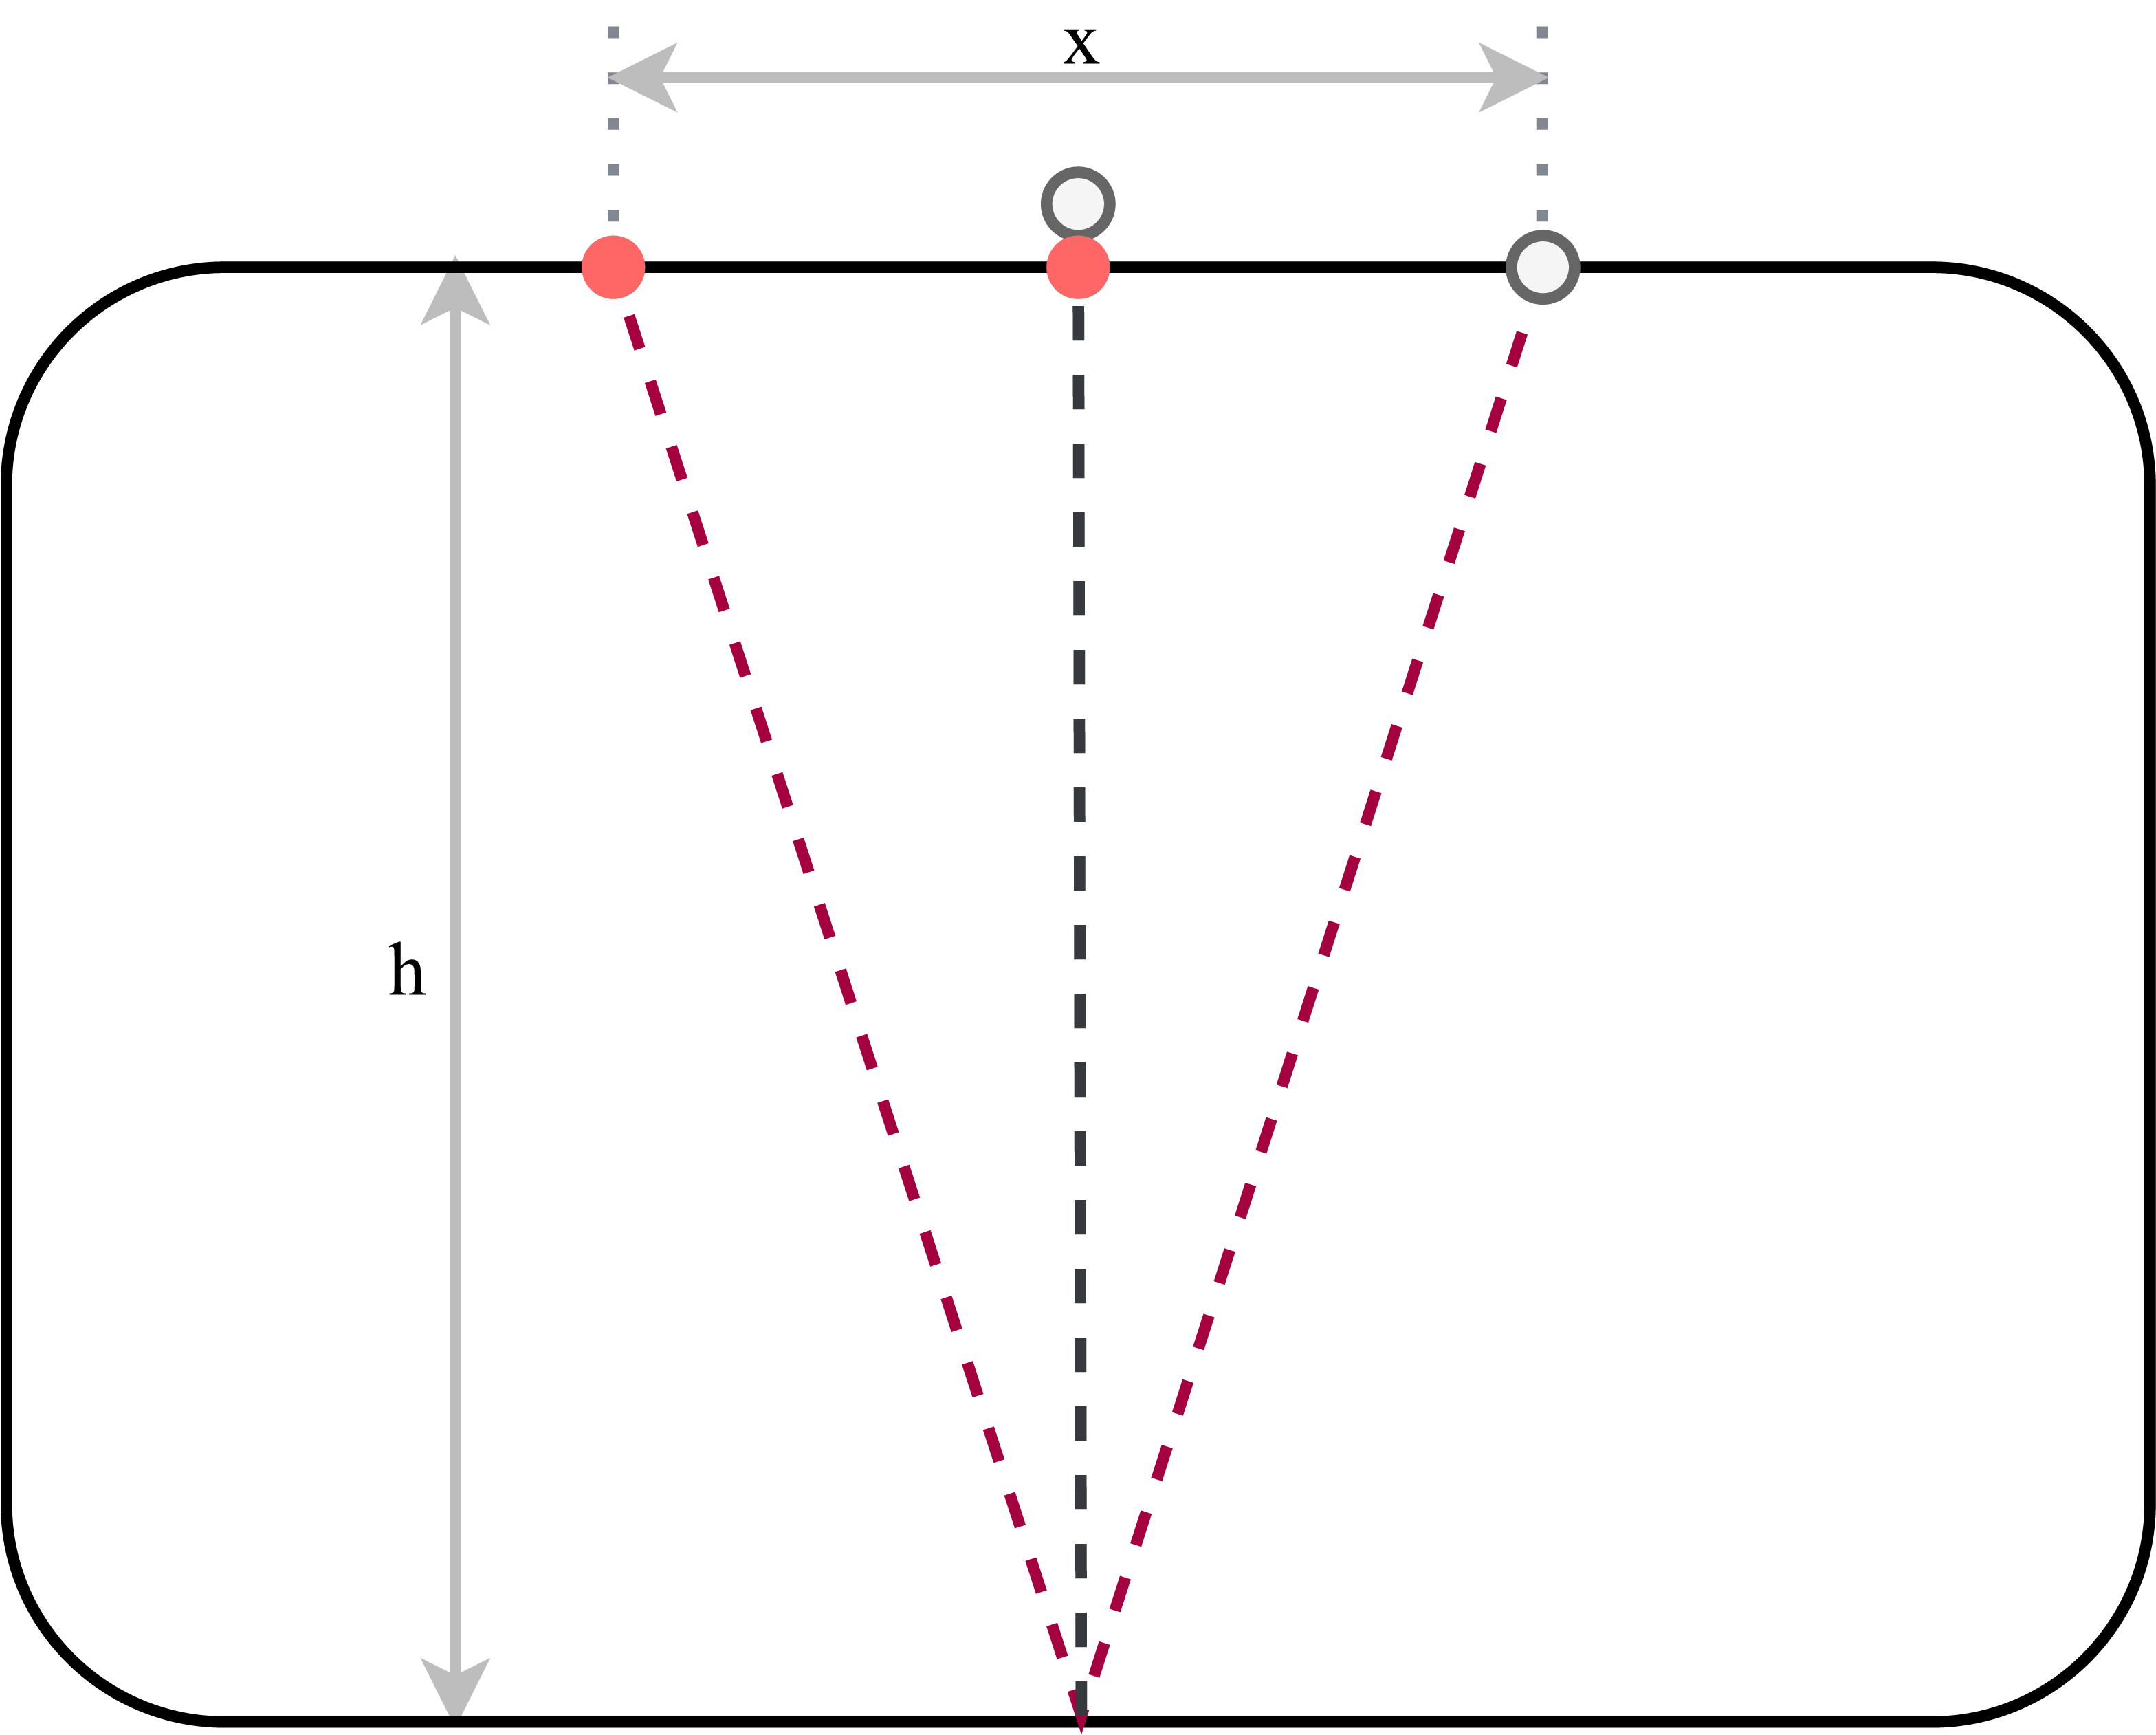
\includegraphics[width = .9\textwidth]{06_旅行时计算公式.png}
        \end{figure}
    \end{minipage}
    \begin{minipage}{.35\paperwidth}
        {\small
        \begin{equation*}
            t=\frac{l}{v}=\frac{2\sqrt{h^2+x^2/4}}{v}, t_0=2h/v, 
        \end{equation*}
        \begin{align*}
            t=\frac{2\sqrt{t_0^2v^2/4+x^2/4}}{v}=\sqrt{t_0^2+\frac{x^2}{v^2}}, 
        \end{align*}
        \begin{equation}
            t_0^2=t^2-\frac{x^2}{v^2}. 
            \label{equ:零偏距旅行时计算公式}
        \end{equation}}
\end{minipage}
\end{frame}

\begin{frame}[c]
    \frametitle{动校正}
    \begin{figure}
        \captionsetup{justification=centering}
        \centering
        \subfigure[]{
        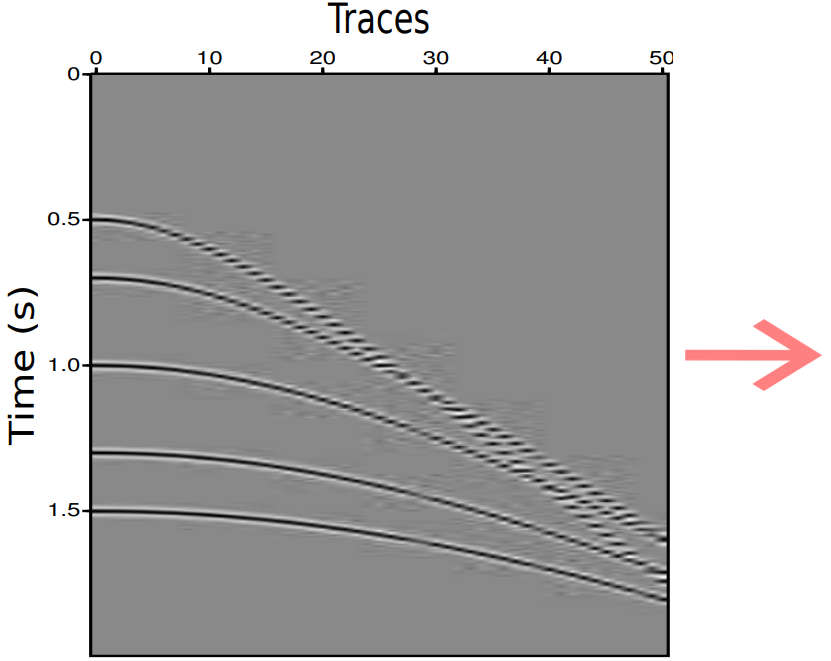
\includegraphics[height=.32\textheight]{555a.png}
        }
        \hspace{-8pt}\subfigure[]{
        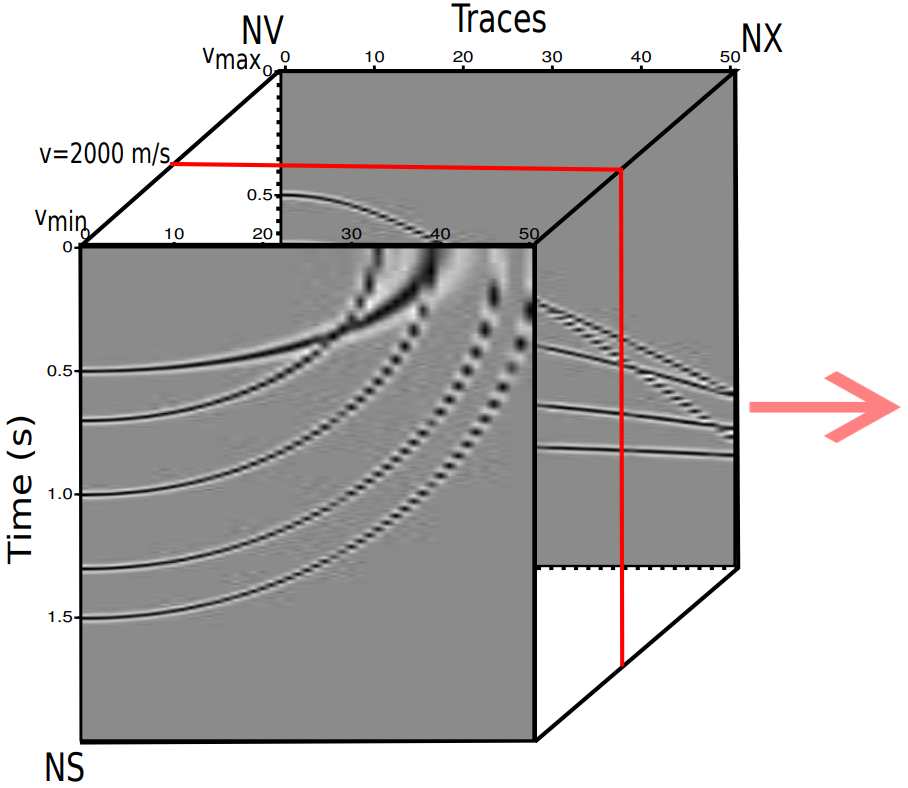
\includegraphics[height=.32\textheight]{555b.png}
        }
        \hspace{-8pt}\subfigure[]{
        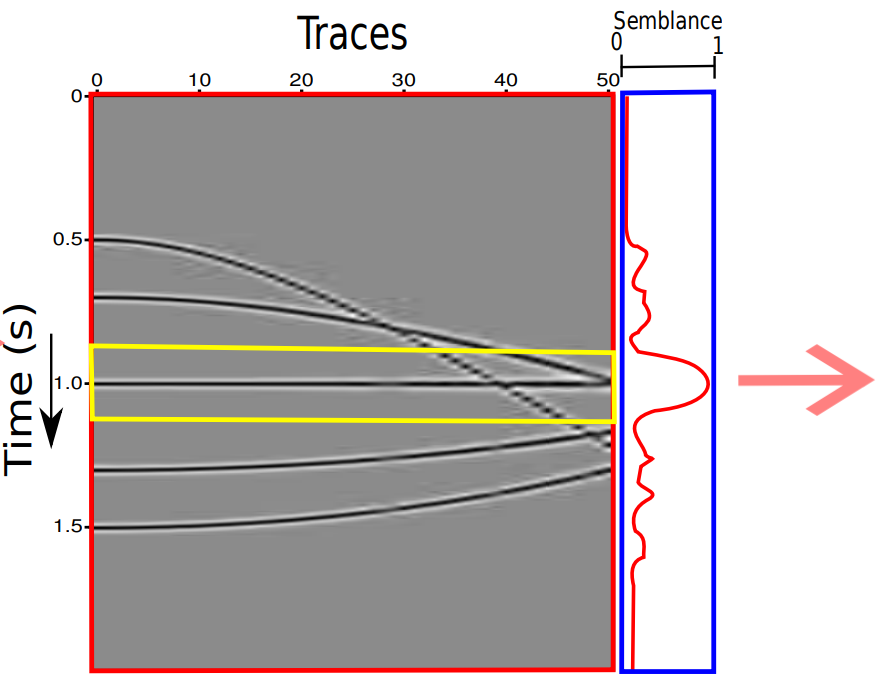
\includegraphics[height=.32\textheight]{555c.png}
        }
        \hspace{-8pt}\subfigure[]{
        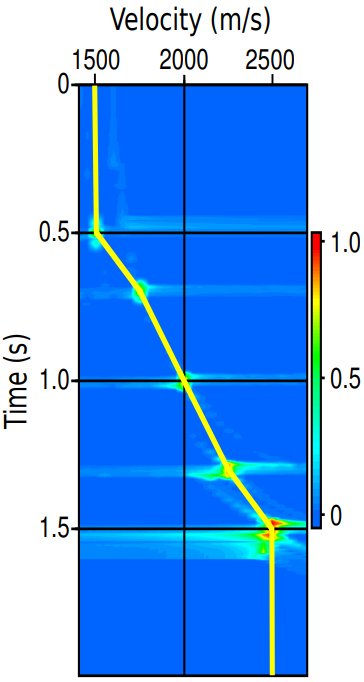
\includegraphics[height=.32\textheight]{555d.png}
        }
        \caption{由5个事件组成的人工CMP道集的速度谱动校正流程。\\(a) CMP道集; (b) 不同速度下的NMO校正结果; \\(c) 速度为2000m/s的NMO校正结果; (d) 速度谱和其各自的速度函数(黄线)\!\!\!。}
    \end{figure}
\end{frame}

% \section{文献阅读、翻译}

% \begin{frame}[c]
%     \frametitle{文献阅读}
%     \vspace{6pt}
%     通过阅读相关的外文文献, 了解到速度分析通常有以下几种方法: 
%         \begin{itemize}
%             \item 速度谱相似性\footfullcite{Gan2016, Chen2015}; 
%             \item 局部地震斜率\footfullcite{Ottolini1983, Fomel2007}; 
%             \item 神经网络\footfullcite{Schmidt1992, Zhang2019, Wang2021}; 
%             \item 聚类\footfullcite{Toldi1989}. 
%         \end{itemize}
% \end{frame}

% \begin{frame}[c]
%     \frametitle{文献翻译}
%     对下列两篇文献\footfullcite{Rodriguez2014, Zhang2016}进行了全文翻译: 
%     \begin{figure}[h]
%         \centering
%         \includegraphics[width=.8\textwidth]{07_article_1.png}\\
%         \includegraphics[width=.8\textwidth]{07_article_2.png}
%     \end{figure}
% \end{frame}

\section{理论知识}

\begin{frame}[c]
    \frametitle{前人工作}
    \vspace{10pt}
    通常对速度分析有以下几种方法: 
        \begin{itemize}
            \item 速度谱相似性(\citeauthor{Gan2016}, \citeyear{Gan2016}); 
            \item 局部地震斜率(\citeauthor{Fomel2007}, \citeyear{Fomel2007}); 
            \item 神经网络(\citeauthor{Wang2021}, \citeyear{Wang2021}); 
            \item 聚类(\citeauthor{Zhang2016}, \citeyear{Zhang2016}). 
        \end{itemize}
\end{frame}

\section{几种常见的聚类算法}

\begin{frame}[c]
    \frametitle{K-means聚类}
    假设我们有$n$个样本$x_1, x_2, \cdots, x_n$, 它们属于$k$个类($S_1,\cdots,S_k$), $k<n$, 则聚类中心$m_i$由以下算法得到

    \vspace{10pt}
    \begin{algorithm}[H]
        \SetAlgoLined
        \KwIn{样本$x_1, x_2, \cdots, x_n$, 聚类中心个数$k$, 终止阈值$\varepsilon$}
        \KwOut{$k$个聚类中心}
        对聚类中心点$m_1, m_2, \cdots, m_k$进行初始化\; 
        \While{聚类中心点的变化不小于阈值$\varepsilon$}{
            将$n$个样本点按照最近原则分配给最近的一个聚类中心\;
            用$m_i=\frac{1}{|S_i|}\sum_{\mathbf{x}\in S_i}\mathbf{x}$计算新的聚类中心\; 
            计算新旧聚类中心点之间的变化量. 
        }
        \caption{K-means聚类}
    \end{algorithm}
\end{frame}

\begin{frame}[c]
    \frametitle{DBSCAN}
    假设我们有$n$个样本$x_1, x_2, \cdots, x_n$, 则DBSCAN算法按照以下步骤实施

    \vspace{10pt}
    \begin{algorithm}[H]
        \SetAlgoLined
        \KwIn{样本$x_1, x_2, \cdots, x_n$, $\varepsilon$邻域半径$Eps$, 最小点数$minPts$}
        \KwOut{每个样本点所属的类}
        找到每个点的$\varepsilon$邻域中的点, 并确定那些邻域内有超过$minPts$个点的核心点\; 
        找到所有与核心点密度可达的点\; 
        将每个核心点和由其密度可达的点划为同一个类, 将其余点划为噪声。
        \caption{DBSCAN}
    \end{algorithm}
\end{frame}

\begin{frame}[c]
    \frametitle{EM算法}
    {\small
    假设我们有$n$个样本$x_1, x_2, \cdots, x_n$, 则基于EM算法的高斯混合模型可以按照以下步骤来实施聚类
    \\\begin{minipage}{.55\textwidth}
        \small
        \begin{equation}
        \label{equ:Complete-Likelihood}
        \begin{aligned}
            &Q(\Theta, \Theta^{(0)})\\ =& E_{Z|X,\Theta^{(0)}}\left (\log (P(X,Z|\Theta)) \right) \\
            =&\int_Z P(Z|X,\Theta^{(0)}) \log (P(X,Z|\Theta))\,\text{d}\,Z, 
        \end{aligned}
        \end{equation}
    \end{minipage}\ 
    \begin{minipage}{.4\textwidth}
        \small
        \begin{equation}
        \label{equ:EM-max}
        \hat{\Theta} = \underset{\Theta}{\arg\max}\ Q(\Theta, \Theta^{(0)}). 
        \end{equation}
    \end{minipage}

    \begin{algorithm}[H]
        \SetAlgoLined
        \KwIn{样本$x_1, x_2, \cdots, x_n$, 聚类中心点个数$k$, 收敛阈值$\varepsilon$}
        \KwOut{$k$个高斯分量的具体参数}
        随机或用特定算法初始化$k$个高斯分量的参数\; 
        \While{似然函数的增长量不小于$\varepsilon$}{
            E(Expectation)步: 用式~\ref{equ:Complete-Likelihood}~计算出关于$Z$的期望估计\; 
            M(Maximization)步: 用式~\ref{equ:EM-max}~对各个参数进行估计\;
            计算似然函数的增长量。
        }
        \caption{基于EM算法的高斯混合模型}
    \end{algorithm}}
\end{frame}

\section{变分推断}

\begin{frame}[c]
    \frametitle{变分推断}
    已知样本$X$, 同时假定此样本被隐变量$Z$所决定, 但我们并不能直接对隐变量实现观测, 只能观测到样本$X$, 需要从样本中有效地推理出隐变量$Z$。
    
    \vspace{10pt}
    可以假设样本服从某个分布$P(X\,)$, 另一方面, 假设隐变量$Z$是服从分布$q(Z\,)$的, 现在我们的目标便是用$q(Z\,)$去逼近真实隐变量$Z$的分布。
\end{frame}

\begin{frame}[c]
    \frametitle{变分推断}
    假定隐变量$Z$各个维度上的分量之间相互独立
    \begin{equation}
        \label{equ:VB-assumption}
        q(Z)=\prod_{i=1}^T q_i(Z_i), 
    \end{equation}

    \pause 将样本$X$的似然函数写为以下形式
    \begin{align}
        \ln (p(X))=\int_{Z}q(Z) \ln& \left(\frac{p(X, Z)}{q(Z)}\right) \,\mathrm{d}\, Z-\int_{Z}q(Z) \ln \left(\frac{p(Z \mid X)}{q(Z)}\right) \,\mathrm{d}\, Z, \\
        &\ln(p(X))=\mathcal{L}(q)+KL(q \| p), 
    \end{align}

    \pause 将式~(\ref{equ:VB-assumption})~中对于$q(Z\,)$的定义带入到$\mathcal{L}(q)$中, 可以获得以下结果
    \begin{equation}
        \label{equ:VB-ELBO}
        \begin{aligned}
            \mathcal{L}(q) &=\int_{Z}q(Z) \ln (p(X, Z)) \,\mathrm{d}\, Z-\int_{Z}q(Z) \ln (q(Z)) \,\mathrm{d}\, Z \\
            &=\underbrace{\int_{Z}\prod_{i=1}^{T} q_{i}\left(Z_{i}\right) \ln (p(X, Z)) \,\mathrm{d}\, Z}_{\text {I}}-\underbrace{\int_{Z}\prod_{i=1}^{T} q_{i}\left(Z_{i}\right) \sum_{i=1}^{T} \ln \left(q_{i}\left(Z_{i}\right)\right) \,\mathrm{d}\, Z}_{\text {II}}. 
        \end{aligned}
    \end{equation}
\end{frame}

\begin{frame}[c]
    \frametitle{变分推断}
    \begin{equation}
    \label{equ:VB-partI}
        \begin{aligned}
            \text{I}=&\int_{Z_n}\cdots\int_{Z_1}\ln(p(X,Z))Tq_i(Z_i)\,\text{d}\,Z_i\\
            =&\int_{Z_j}q_j(Z_j)\left(\underset{i\not=j}{\int\cdots\int}\ln(p(X,Z))\prod_{i\not=j}^Tq_i(Z_i)\,\text{d}\,Z_i\right)\,\text{d}\,Z_j, \\
            \pause=&\int_{Z_{j}} q_{j}\left(Z_{j}\right)\left(\underset{i\not=j}{E_{q_i(Z_i)}}(\ln (p(X, Z)))\right) \,\text{d}\, Z_{j}. 
        \end{aligned}
    \end{equation}
\end{frame}

\begin{frame}[c]
    \frametitle{变分推断}
    {\small
    \begin{equation*}
        \begin{aligned}
            \text{II}=&\int_Z \prod_{i=1}^{T} q_{i}\left(Z_{i}\right) \sum_{i=1}^{T} \ln \left(q_{i}\left(Z_{i}\right)\right) \,\text{d}\, Z\\
            =&\int_{Z_n\cdots Z_1}\left(q_1(Z_1)\prod_{i=2}^Tq_i(Z_i)\left(\ln(q_1(Z_1))+\sum_{i=2}^T\ln(q_i(Z_i))\right)\right)\,\text{d}\,Z_1\cdots Z_n\\\pause
            =&\int_{Z_n\cdots Z_1}\left(q_1(Z_1)\prod_{i=2}^Tq_i(Z_i)\ln(q_1(Z_1))+q_1(Z_1)\prod_{i=2}^Tq_i(Z_i)\sum_{i=2}^T\ln(q_i(Z_i))\right)\,\text{d}\,Z_1\cdots Z_n\\\pause
            =&\int_{Z_1}q_1(Z_1)\ln(q_1(Z_1))\,\text{d}\,Z_1+\int_{Z_n\cdots Z_2}\prod_{i=2}^Tq_i(Z_i)\sum_{i=2}^T\ln(q_i(Z_i))\,\text{d}\,Z_2\cdots Z_n\\\pause
            =&\sum_{i=1}^T\left(\int_{Z_i}q_i(Z_i)\ln(q_i(Z_i))\,\text{d}\,Z_i\right), 
        \end{aligned}
    \end{equation*}}
\end{frame}

\begin{frame}[c]
    \frametitle{变分推断}
    与对I部分所做操作一样, 也将II部分中的分量$Z_j$独立出来, 按照假设, 各个分量是独立的, 因此其他分量的积分结果是常数, 即
    \begin{equation}
        \label{equ:VB-partII}
        \text{II}=\int_{Z_j}q_j(Z_j)\ln(q_j(Z_j))\,\text{d}\,Z_j+C, 
    \end{equation}

    其中, $C$是与$Z_j$无关的常数。
\end{frame}

\begin{frame}[c]
    \frametitle{变分推断}
    将式~(\ref{equ:VB-partII})~与式~(\ref{equ:VB-partI})~代回到式~(\ref{equ:VB-ELBO})~中, 得到
    \begin{equation}
        \label{equ:VB-ELBO2}
        \mathcal{L}(q)=\int_{Z_{j}} q_{j}\left(Z_{j}\right)\left(\underset{i\not=j}{E_{q_i(Z_i)}}\left(\ln (p(X, Z))\right)\right)\text{d}\, Z_{j}-\int_{Z_j}q_j(Z_j)\ln(q_j(Z_j))\,\text{d}\,Z_j+C. 
    \end{equation}

    \pause 可以注意到$\underset{i\not=j}{E_{q_i(Z_i)}}\left(\ln (p(X, Z))\right)$将会是$Z_j$的一个函数, 因此作出以下定义
    \begin{equation}
        \ln \left(\tilde{p}_{j}\left(X, Z_{j}\right)\right)\triangleq\underset{i\not=j}{E_{q_i(Z_i)}}\left(\ln (p(X, Z))\right), 
    \end{equation}
    
    \pause 从而, 可以得到式~(\ref{equ:VB-ELBO2})~的化简形式: 
    \begin{equation}
        \label{equ:VB-ELBO3}
        \mathcal{L}(q_j)=\int_{Z_j}q_j(Z_j)\ln\left(\frac{\tilde{p}_{j}\left(X, Z_{j}\right)}{q_j(Z_j)}\right)\text{d}\,Z_j+C. 
    \end{equation}
\end{frame}

\begin{frame}[c]
    \frametitle{变分推断}
    可以看到, 除去常数项, 式~(\ref{equ:VB-ELBO3})~实际上是两个分布的$KL$散度取负值, 即
    \[-KL\left(q_j(Z_j)\|\tilde{p}_{j}\left(X, Z_{j}\right)\right), \]
    \pause 对每个分量$q_j$分别计算, 从而实现$ELBO$的最大化, $q_j(Z_j)$的取值如下
    \begin{equation}
        \begin{aligned}
            q_j(Z_j)=\tilde{p}_{j}\left(X, Z_{j}\right)=\exp\left(\underset{i\not=j}{E_{q_i(Z_i)}}\left(\ln (p(X, Z))\right)\right), 
        \end{aligned}
    \end{equation}
    \pause 或者也可以写为
    \begin{equation}
        \ln(q_j(Z_j))=\underset{i\not=j}{E_{q_i(Z_i)}}\left(\ln (p(X, Z))\right). 
    \end{equation}
    这样, 我们通过迭代地对$Z_1,\cdots,Z_n$进行更新, 从而估计出$q(Z\,)$的分布。
\end{frame}

\section{Dirichlet过程}

\begin{frame}[c]
    \frametitle{背景}
    对于模型参数$\Theta$的先验去选取一个连续的分布, 任何两个不同的样本点$x_i, x_j$, 它们各自所属分布的参数$\theta_i, \theta_j$也会不同。

    \pause{}若有$n$个样本点, 得到$n$个参数分别为$\theta_1,\cdots,\theta_n$的互不相同的分布, 这样虽然实现了对于分布分量参数的确定, 但却是没有实际应用价值的。

    \pause{}因此, 就需要为$\Theta$定义一个离散的先验分布, 从而使得估计出的某一部分样本点所属分布的参数$\theta_i$都具有相同的值。
    
    \pause{}还希望这个离散的分布可以更好的近似$\Theta$真正的分布。而从Dirichlet过程中抽样出的一个分布就契合所要寻找的那个离散分布。
\end{frame}

\begin{frame}[c]
    \frametitle{Dirichlet过程}
    令$\Omega$表示样本空间, $G_0$表示在样本空间上的一个分布函数, $\alpha$是一个正实数
    
    若存在一个随机的分布函数$G$, 对于样本空间$\Omega$的任意一个的可测划分$(A_1$, $A_2$, $\cdots$, $A_k)$, 满足
    \[\left(G(A_1), G(A_2), \cdots, G(A_k)\right)\sim Dir\left(\alpha G_0(A_1), \alpha G_0(A_2), \cdots, \alpha G_0(A_k)\right), \]
    则称这个随机分布$G$是服从以$\alpha$为尺度参数, $G_0$为基础分布的Dirichlet过程, 即
    \[G\sim DP(\alpha, G_0). \]
\end{frame}

\begin{frame}[c]
    \frametitle{Dirichlet Process Mixtures}
    \begin{figure}[ht]
        \centering
        \begin{tikzpicture}
        \tikzstyle{main}=[circle, minimum size = 10mm, thick, draw =black!80, node distance = 8mm]
        \tikzstyle{connect}=[-latex, thick]
        \tikzstyle{box}=[rectangle, draw=black!100]
            \node[main] (alpha) {$\alpha$};
            \node[node distance =4mm] (temp) [below=of alpha] {};
            \node[main, node distance =4mm] (Base) [below=of temp] {$G_0$};
            \node[main] (DPSample) [right=of temp] {$G$};
            \node[main] (theta) [right=of DPSample] {$\theta_i$};
            \node[main] (data) [right=of theta] {$x_i$};
            \path (alpha) edge [connect] (DPSample)
                        (Base) edge [connect] (DPSample)
                        (DPSample) edge [connect] (theta)
                        (theta) edge [connect] (data); 
            \node[rectangle, inner sep=0mm, fit= (theta) (data), label=below right:N, xshift=7mm, yshift=1.5mm] {};
            \node[rectangle, inner sep=3.5mm,draw=black!100, fit= (theta) (data)] {};
        \end{tikzpicture}
        % \caption{Dirichlet过程混合模型概率图。\label{fig:dirichlet-ppm}}
    \end{figure}

    \begin{align*}
        G & \sim DP\left(\alpha, G_{0}\right); \\
        \theta_{i} & \sim G; \\
        x_{i} & \sim p\left(x_{i} \mid \theta_{i}\right). 
    \end{align*}
\end{frame}

\begin{frame}[c]
    \frametitle{性质}
    \[E(G(A_i))=\frac{\alpha G_0(A_i)}{\sum_j \alpha G_0(A_j)}=G_0(A_i), \]
    \begin{align*}
        Var(G(A_i))=&\frac{\alpha G_0(A_i)\left(\alpha-\alpha G_0(A_i) \right)}{\alpha^2(\alpha+1)}\\=&\frac{G_0(A_i)(1-G_0(A_i))}{\alpha+1}. 
    \end{align*}
\end{frame}

\begin{frame}[c]
    \frametitle{Stick-Breaking}
    对于想要构造出的离散分布$G$, 我们可以将其表示为以下形式
    \begin{equation}
        G=\sum_{i=1}^{\infty}\pi_{i}\delta_{\theta_i}(\theta), 
    \end{equation}

    \begin{equation}
        \begin{aligned}
            \pause 
            &\beta_1, \beta_2, \cdots, \beta_k, \cdots \overset{i.i.d.}\sim Beta(1,\alpha); \\
            \pause 
            &\pi_1=\beta_1; \\
            \pause 
            &\pi_j=\beta_j(1-\sum_{i=1}^{j-1} \pi_i)=\beta_j\prod_{i=1}^{j-1}(1-\beta_i), (j>1); \\
            \pause 
            &G(\theta)=\sum_{i=1}^{\infty}\pi_i\delta_{\theta_i}(\theta). 
        \end{aligned}
    \end{equation}
\end{frame}

\begin{frame}[c]
    \frametitle{Dirichlet过程的变分推断}
    变分推断在Dirichlet过程上的计算相对复杂, 但好在\citeauthor{Blei2006}(\citeyear{Blei2006})用坐标上升法给出了变分推断对一般指数族的Dirichlet过程混合模型的参数迭代公式。
    
    E步: 
    \begin{equation}
        \label{equ:qwiueiqwhe}
        E_{q}\left[\log p\left(Z_{n} \mid \boldsymbol{\beta}\right)\right]=\sum_{i=1}^{T} q\left(z_{n}>i\right) E_{q}\left[\log \left(1-\beta_{i}\right)\right]+q\left(z_{n}=i\right) E_{q}\left[\log \beta_{i}\right], 
    \end{equation}
    其中
    {\small
    \begin{equation*}
        \begin{aligned}
            &q\left(z_{n}=i\right) =\phi_{n, i}, \ q\left(z_{n}>i\right) =\sum_{j=i+1}^{T} \phi_{n, j}, \\
            &E_{q}\left[\log \beta_{i}\right] =\Psi\left(\gamma_{i, 1}\right)-\Psi\left(\gamma_{i, 1}+\gamma_{i, 2}\right), \\
            &E_{q}\left[\log \left(1-\beta_{i}\right)\right] =\Psi\left(\gamma_{i, 2}\right)-\Psi\left(\gamma_{i, 1}+\gamma_{i, 2}\right), 
        \end{aligned}
    \end{equation*}
    }
    $\Psi$表示digamma函数, $\gamma_{t}$是贝塔分布。
\end{frame}

\begin{frame}[c]
    \frametitle{Dirichlet过程的变分推断}
    
    M步: 之后, 用坐标上升法得到以下迭代公式。

    \begin{equation}
        \label{equ:asduaisdawqdh}
        \begin{aligned}
        \gamma_{t, 1} &=1+\sum_{n} \phi_{n, t};&
        \gamma_{t, 2} =\alpha+\sum_{n} \sum_{j=t+1}^{T} \phi_{n, j}; \\
        \tau_{t, 1} &=\lambda_{1}+\sum_{n} \phi_{n, t} x_{n};& 
        \tau_{t, 2} =\lambda_{2}+\sum_{n} \phi_{n, t}; \\
        \phi_{n, t} & \propto \exp \left(S_{t}\right). &
        \end{aligned}
    \end{equation}
    在满足条件$t \in\{1, \ldots, T\}$和$n \in\{1, \ldots, N\}$时, 有: 
    \begin{equation*}
        S_{t}=E_{q}\left[\log \beta_{T}\right]+\sum_{i=1}^{t-1} E_{q}\left[\log \left(1-\beta_{i}\right)\right]+E_{q}\left[\theta_{t}^{*}\right]^{T} X_{n}-E_{q}\left[a\left(\theta_{t}^{*}\right)\right]. 
    \end{equation*}
\end{frame}

\begin{frame}[c]
    \frametitle{Dirichlet过程的变分推断}
    \begin{algorithm}[H]
        \SetAlgoLined
        \KwIn{样本$x_1, x_2, \cdots, x_n$, 收敛阈值$\varepsilon$, 预先指定的聚类中心个数上限$t$. }
        \KwOut{$t$个高斯分量的具体参数}
        随机或用特定算法初始化$t$个高斯分量的参数\; 
        \While{似然函数的增长量不小于$\varepsilon$}{
            E(Expectation)步: 用式~\ref{equ:qwiueiqwhe}~计算出关于$Z$的期望估计\; 
            M(Maximization)步: 用式~\ref{equ:asduaisdawqdh}~对各个参数进行估计\; 
            计算似然函数的增长量。
        }
        \caption{基于Dirichlet过程的高斯混合模型}
    \end{algorithm}
\end{frame}

\section{数值实验}

% \begin{frame}[c]{代码编写}
%     \begin{itemize}
%         \item 代码共计约1000行; 
%         \vspace{10pt}\item 实现了对地震数据进行读取、预处理、聚类、结果分析、曲线拟合、在原始道集上进行动校正的功能.
%         \vspace{10pt}\item 聚类部分的代码可以在此Github仓库\footnote{\tiny https://github.com/Addasecond86/XJTU-Bachelor-Dissertation-Statistics-WangZehao/tree/main/codes}中查看. 
%     \end{itemize}
% \end{frame}

\begin{frame}[c]
    \frametitle{DBSCAN试验结果}
    \begin{figure}[ht]
        \captionsetup{justification=centering}
        \centering
        \subfigure[Eps=0.015, minPts=2, n=67]{
            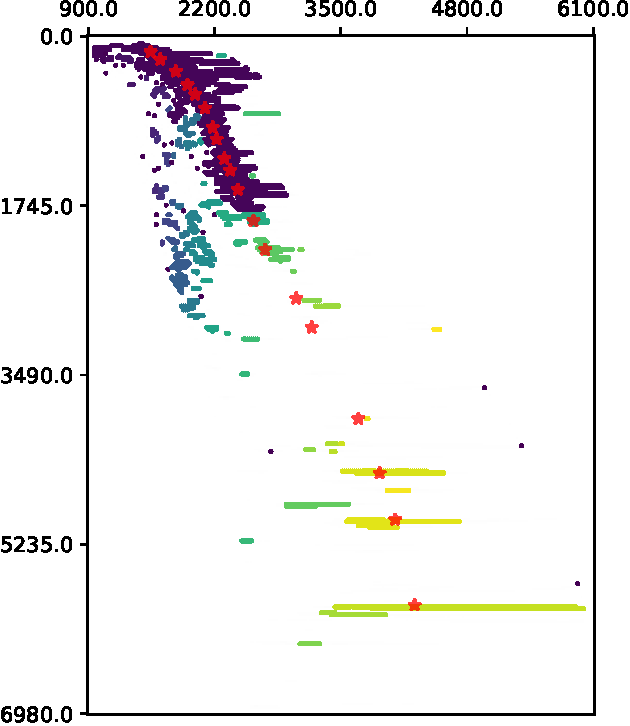
\includegraphics[height=6cm]{10_DBSCAN_Raw_Normalized=True_Threshold=0.01_TruePair_ResultPoint_ClusterNumber=67_Eps=0.025_MSA=2.pdf}
        }\ 
        \subfigure[Eps=0.015, minPts=4, n=0]{
            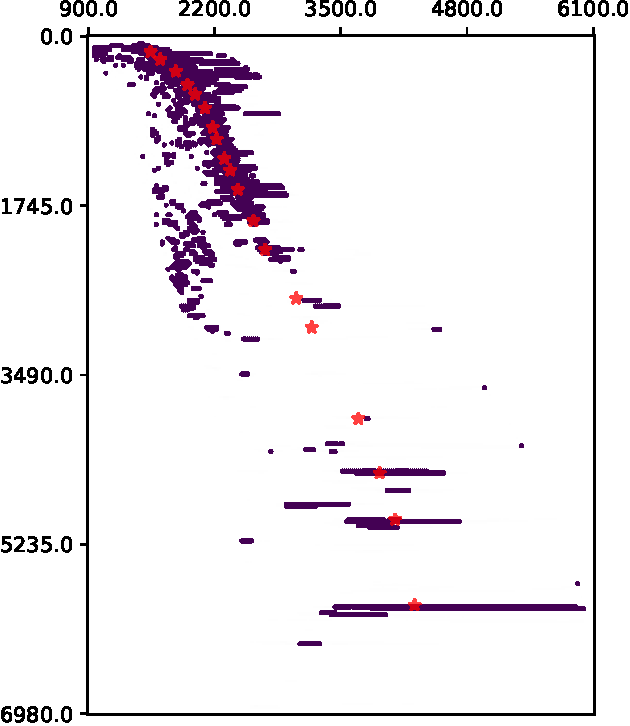
\includegraphics[height=6cm]{11_DBSCAN_Raw_Normalized=True_Threshold=0.01_TruePair_ResultPoint_ClusterNumber=0_Eps=0.015_MSA=4.pdf}
        }
    \end{figure}
\end{frame}

\begin{frame}[c]
    \frametitle{K-means试验结果}
    \begin{figure}[ht]
        \captionsetup{justification=centering}
        \centering
        \hspace{20pt}\subfigure[原始数据点的划分]{
            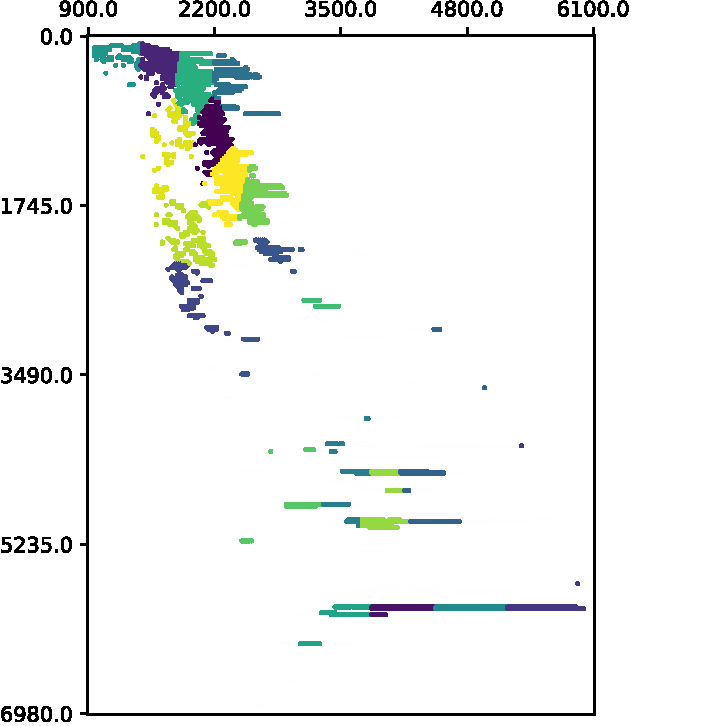
\includegraphics[height=5.8cm]{09_K-means_Raw_Normalized=True_Threshold=0.01_ResultPoint_ClusterNumber=20.pdf}
        }\ 
        \hspace{-20pt}\subfigure[聚类中心]{
            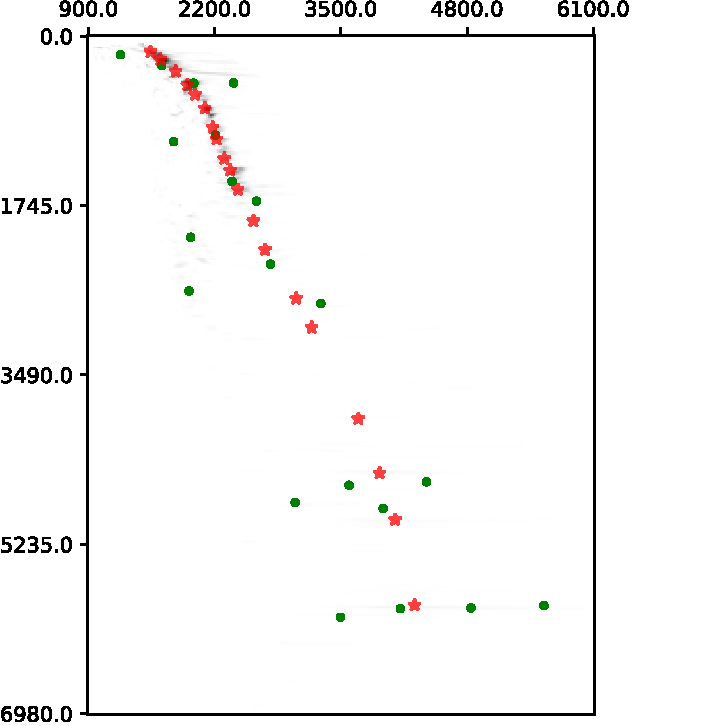
\includegraphics[height=5.8cm]{09_K-means_Raw_Normalized=True_Threshold=0.01_TruePair_Centers_n=20.pdf}
        }
    \end{figure}
\end{frame}

\begin{frame}[c]
    \frametitle{GMM-EM试验结果}
    \captionsetup{justification=centering}
    \begin{figure}[ht]
        \captionsetup{justification=centering}
        \centering
        \subfigure[指定聚类中心个数: 15]{
            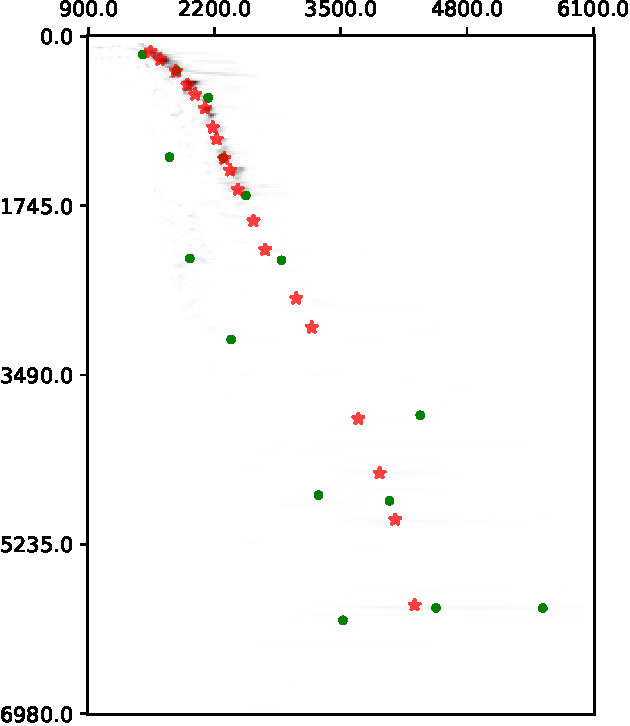
\includegraphics[height=5.8cm]{12_GMM_EM_Raw_Normalized=True_Threshold=0.01_TruePair_Centers_n=15_CovType=diag.pdf}
        }
        \subfigure[指定聚类中心个数: 20]{
            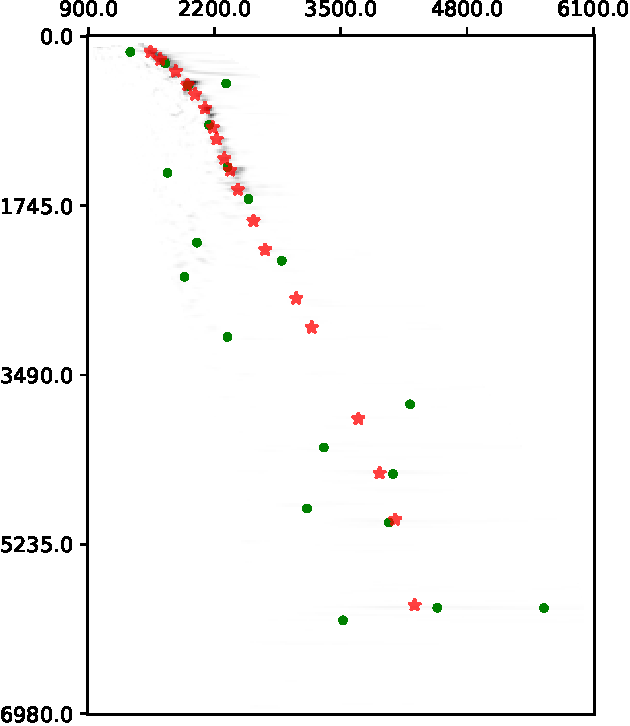
\includegraphics[height=5.8cm]{12_GMM_EM_Raw_Normalized=True_Threshold=0.01_TruePair_Centers_n=20_CovType=diag.pdf}
        }
    \end{figure}
\end{frame}

\begin{frame}[c]
    \frametitle{GMM-DP试验结果}
    \begin{figure}[ht]
    \captionsetup{justification=centering}
        \centering
        \subfigure[设置: 10, 实际: 10]{
            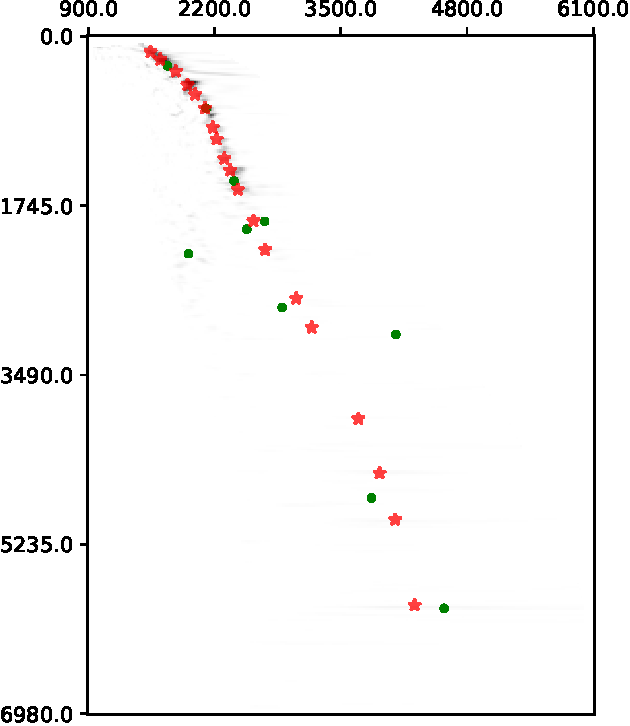
\includegraphics[height=5.8cm]{14_GMM_Dirichlet_Raw_Normalized=True_Threshold=0.01_TruePair_Centers_Real_n=10_n=10_CovType=diag_PriorType=dirichlet_process_Prior=0.1.pdf}
        }
        \subfigure[设置: 35, 实际: 11]{
            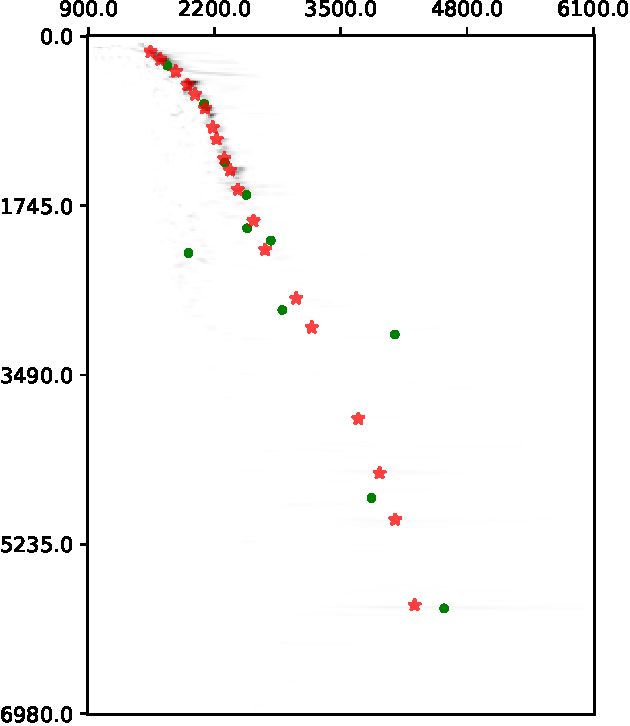
\includegraphics[height=5.8cm]{14_GMM_Dirichlet_Raw_Normalized=True_Threshold=0.01_TruePair_Centers_Real_n=35_n=11_CovType=diag_PriorType=dirichlet_process_Prior=0.03.pdf}
        }
    \end{figure}
\end{frame}

\begin{frame}[c]
    \frametitle{GMM-DP试验结果}
    预先指定的聚类中心个数在大于一定范围后上对结果不造成影响!
    
    \vspace{10pt}\begin{table}[h]
        \begin{tabular}{cc}
        \hline
        预先指定的聚类中心上限个数 & 实际结果 \\ \hline
        10          & 10   \\
        15          & 10   \\
        20          & 11   \\
        25          & 11   \\
        30          & 11   \\
        35          & 11   \\ \hline
        \end{tabular}
    \end{table}
\end{frame}

\begin{frame}[c]
    \frametitle{曲线拟合}
    \begin{figure}[ht]
        \captionsetup{justification=centering}
        \centering
        \subfigure[结合一部分K-means后的结果]{
            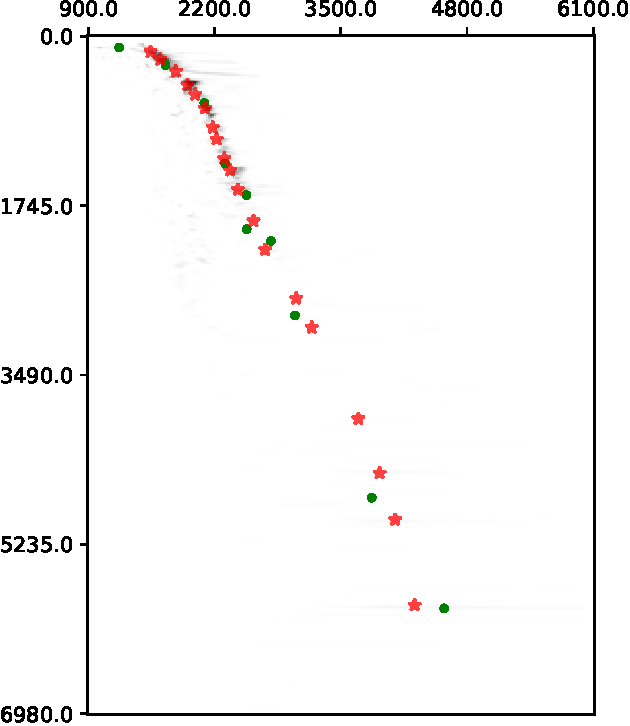
\includegraphics[height=5.8cm]{15_GMM_Dirichlet_TruePair_Centers_Real_n=35_n=9_CovType=diag_PriorType=dirichlet_process_Prior=0.03.pdf}
        }
        \subfigure[所拟合出的曲线]{
            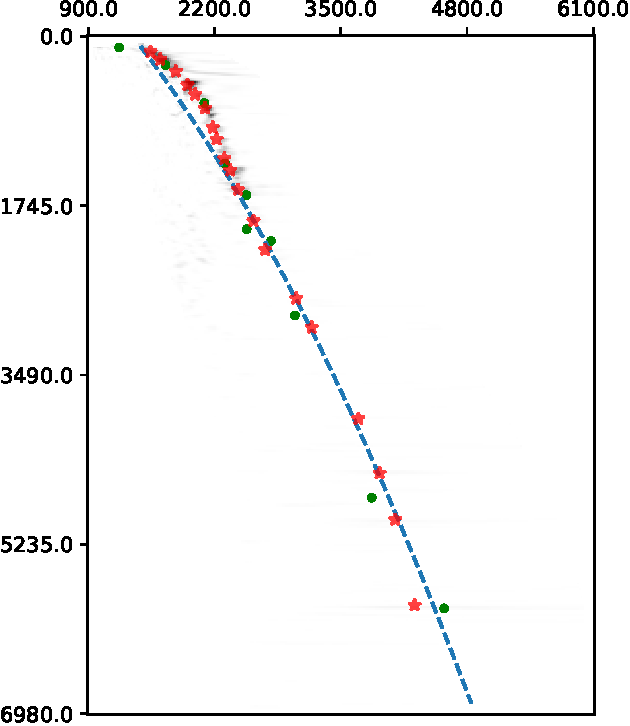
\includegraphics[height=5.8cm]{16_GMM_Dirichlet_FittingMethod=Square_Curve_TruePair_Centers_Real_n=35_n=10_CovType=diag_PriorType=dirichlet_process_Prior=0.03_NoCombine.pdf}
        }
    \end{figure}
\end{frame}

\begin{frame}[c]
    \frametitle{对原始道集进行动校正}
    \begin{figure}[ht]
        \captionsetup{justification=centering}
        \centering
        \subfigure{
            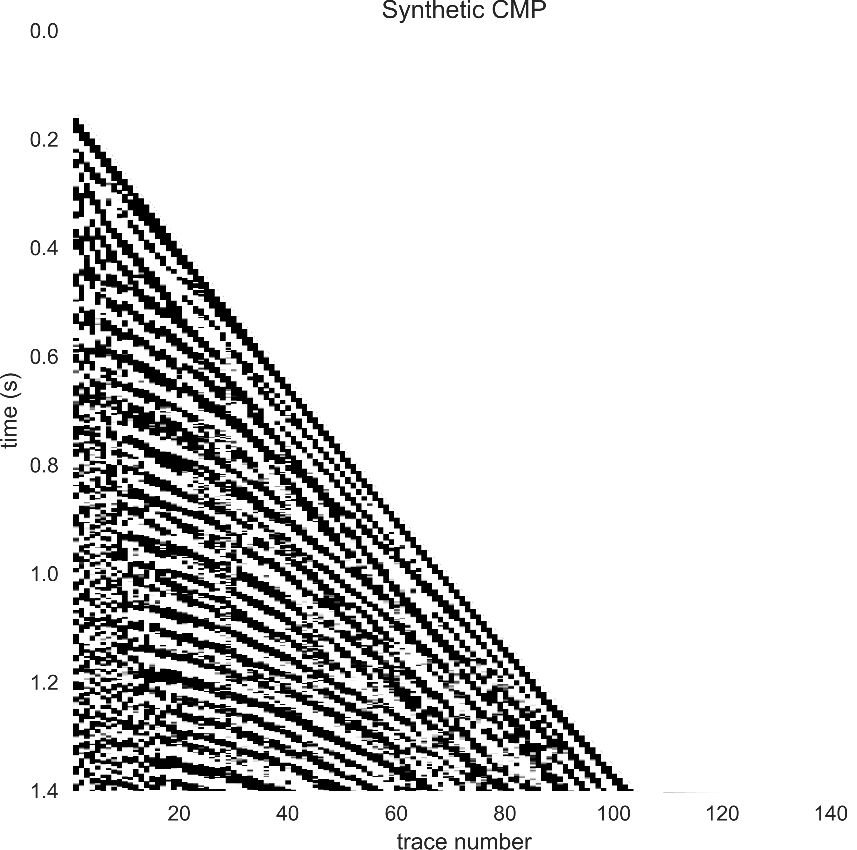
\includegraphics[width=.45\textwidth]{17_0.8_1.4_原始道集.pdf}
        }
        \subfigure{
            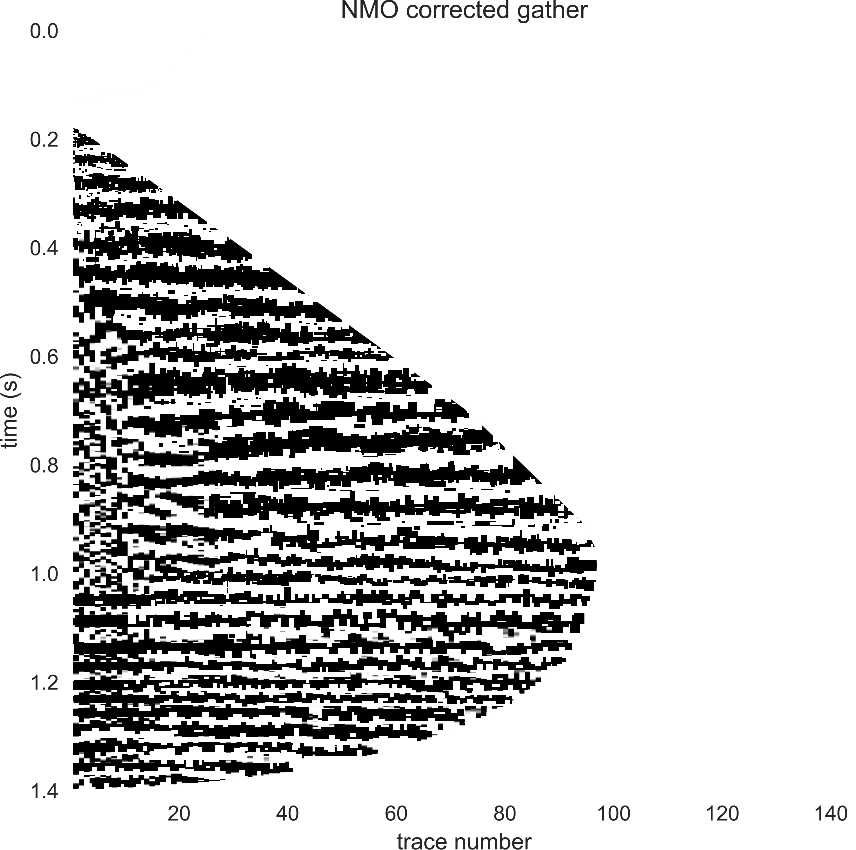
\includegraphics[width=.45\textwidth]{17_0.8_1.4_NMO.pdf}
        }
    \end{figure}
\end{frame}

\section{结论与展望}

\begin{frame}[c]
    \frametitle{结论}
    基于 Dirichlet 过程的高斯混合模型在地震速度谱自动拾取的问题上能发挥较为良好的性能, 主要表现在: 
    
    \vspace{10pt}\begin{itemize}
        \item 不需要预先确定聚类中心个数; 
        \vspace{10pt}\item 所的聚类结果对原始道集的拉直效果良好. 
    \end{itemize}
\end{frame}

\begin{frame}[c]
    \frametitle{展望}
    后续可以考虑以下改进方向: 
    \begin{center}
        \begin{minipage}{.75\textwidth}
            \begin{enumerate}
                \vspace{10pt}\item 探究更为合理的曲线拟合方法; 
                \pause\vspace{10pt}\item 探究更加有效剔除噪声的方法. 
            \end{enumerate}
        \end{minipage}
    \end{center}
\end{frame}

\begin{frame}[plain]
    \printbibliography
\end{frame}

\section*{谢谢各位老师!}
\end{document}
